
%(BEGIN_QUESTION)
% Copyright 2006, Tony R. Kuphaldt, released under the Creative Commons Attribution License (v 1.0)
% This means you may do almost anything with this work of mine, so long as you give me proper credit

Sketch a ladder logic diagram for a simple baking oven temperature control circuit with three temperature switches.  One switch will be a high-temperature alarm which turns on a lamp if the temperature exceeds 450$^{o}$ F.  Another switch will control power to the heating element, turning it on if the temperature is below 350$^{o}$ F.  The last switch will activate a ``pre-heating'' indication lamp, to tell the cook when the oven is not yet at its operating temperature (any temp below 310$^{o}$ F).

$$\includegraphics[width=15.5cm]{i00648x01.eps}$$

\vskip 10pt

\noindent
Credit will be given for correctly wiring each of the three branch circuits.  You {\it must} write the given temperature setting (in degrees F) next to each switch in order to receive credit for that circuit:

\begin{itemize}
\item{} High temperature alarm lamp
\item{} Heater control
\item{} ``Pre-heating'' lamp
\end{itemize}

\underbar{file i00648}
%(END_QUESTION)





%(BEGIN_ANSWER)

$$\includegraphics[width=15.5cm]{i00648x02.eps}$$

4 points for heating element switch, 3 points for each of the others.

%(END_ANSWER)





%(BEGIN_NOTES)

{\bf This question is intended for exams only and not worksheets!}.

%(END_NOTES)


